\documentclass[ukenglish]{nik}  

%NIK packages
\usepackage{times}

\usepackage[latin1]{inputenc}
%angir tegnsettet i LaTeX-filen. (Opsjonen m� selvf�lgelig tilpasses om man har et annet tegnsett.)
\usepackage[T1]{fontenc}
%spesifiserer bruk av 8-bits fonter.
%\usepackage{babel}  only needed for Norwegian I suppose
%ordner alle spr�kavhengig ting.
\usepackage{textcomp}
%gir tilgang til flere symboler.
\usepackage{type1cm}
%forteller at systemet kan skalere Computer Modern i alle st�rrelser. 	

%Spesific packages
\usepackage{geometry}    
\usepackage{graphicx}				
\usepackage{array}								
\usepackage{amssymb}
\usepackage{cite}





\title{Requirement Engineering Process in AMIDST}
\author{The handsome AMIDST guys et. al.}
\date{Latest version, \today}							% Activate to display a given date or no date

\begin{document}
\maketitle
%
%\begin{abstract}
%\end{abstract}
%
\section{Introduction}

Despite the fact that the field of requirement engineering RE has existed since the seventies, very few surveys have been conducted on RE for very small software projects with less than 10 developers \cite{Qui10}. In 2007, a study of seven very small software enterprises in Canada was conducted \cite{Ara07}.
And in 2011, a study which involved 24 experienced project managers from 24 different small software companies in Chile was conducted \cite{Qui10}.  Based on these two studies, it is clear that RE processes in very small companies are more ad-hoc and that there seem to be little agreement on how to conduct the RE process in practice.

In the literature, several ready-to-use approaches for RE on small projects are attempted.  In 2004, Nikula presented a basic RE model baRE as part of his PhD thesis \cite{Nik04}.  Based on an argumentation in \cite{Qui10}, this method may not be suitable for very small projects, because the method is based on results from a study that involved mostly larger companies \cite{Nik00}.   Dorr et. al. presented a set of 36 RE practices for RE improvement for small software projects \cite{Dor08}.  However, the six companies that was considered had between 20 and 200 employees, meaning that this research was also biased towards medium sized projects rather than very small. 

It is also worth mentioning that a large portion of modern software companies follows Agile methods for software development \cite{Din10}.  Paper \cite{Kav11} outlines how to incorporate requirement gathering in small Agile projects.  However, in the Agile methodology, requirement engineering is seen as an ongoing process throughout the whole project, which involves a product owner that continuously renegotiates the requirements.  Due to the project management process in EU's Seventh Framework Programme, the AMIDST project is limited from following such a process. 

Based on the lack of clarity in practice and consensus in literature on a common RE process for small projects, we decided to identify the characteristics of our project and motivate our choices related to the RE process from this.  For instance, the AMIDST project is characterized by the fact that there is a description of work that is agreed upon upfront.  The 
AMIDST RE process must comply with the STREP proposal FP7-ICT-2013-11, and the software must comply with all deliveries in work package 1 to 8. 
%task 2.3 in work package 2, tasks; 3.3, 3.4, 3.5, 3,6 and 3.7 in work package 3, tasks; 4.1, 4,2 4,3 and 4.4 in work package 4 and tasks; 5.1, 5,3, 5,4 and 5,6 in work package 5.

Another important characteristic, is that there is a huge widespread of stakeholders in the project and that the software is required to interface with three different softwares from three different companies.  Because of this, we chose to focus on the functional requirements, which are the requirements that are the most transparent to the user.  As will be discussed later, a use case driven approach \cite{Poh10} and \cite{Coc01} is taken to achieve this.

The report is outlined as follows.  In section \ref{sec:stateOfArt}, the basic principles of requirement engineering are briefly outlined.  Section \ref{sec:AmidstRequirementProcess} starts by describing the main characteristics of the AMIDST project, before the RE process is outlined.  In section \ref{sec:realization}, we have described the realization of the process so far, before the report is concluded in section \ref{sec:conclusion}.

\section{Basic principles in requirement engineering}
\label{sec:stateOfArt}

In practice, the requirement engineering process ends with a document containing a list with requirements, which are in the form of what a software must do or comply with.  

To date there is no common definition of requirement engineering.  Some definitions focus on elicitation of requirements and therefore the interaction with the user, while others focus on the documentation or the specification.  A definition that takes both focuses into account is the IEEE standard given in \cite{Iee90}:

\emph{
\begin{enumerate}
\item The process of studying user needs to arrive at a definition of system, hardware or software requirements.
\item The process of studying and refining system, hardware or software requirements.
\end{enumerate}
}

In the context of understanding the requirement engineering process, it is worth spending some space on defining the requirement itself.  A definition of a requirement is given in IEEE standard \cite{Iee90}: 
\emph{
\begin{enumerate}
\item A condition or capability needed by a user to solve a problem or achieve an objective. 
\item A condition or capability that must be met or possessed by a system or system component to satisfy a contract, standard, specification or other formally imposed document. 
\item A documented representation of a condition or capability as in 1 or 2.
\end{enumerate}
}

This definition has a clear focus on the user, the system/system component and also which contract, standard or specification is needed to be met. Notice, that the requirement is related to \emph{what} a system can do and not \emph{how} it is done.

\subsection{Activities involved in requirement engineering}

The activities involved in requirements engineering vary widely, depending on the type of system being developed and the specific practices of the organization(s) involved  \cite{Som11}.  These may include:
\begin{itemize}
\item Requirements inception or requirements elicitation 
\item Requirements identification - identifying new requirements
\item Requirements analysis and negotiation - checking requirements and resolving stakeholder conflicts
\item Requirements specification (Software Requirements Specification) - documenting the requirements in a requirements document
\item System modeling - deriving models of the system, often using a notation such as the Unified Modeling Language
\item Requirements validation - checking that the documented requirements and models are consistent and meet stakeholder needs
\item Requirements management - managing changes to the requirements as the system is developed and put into use
\end{itemize}

These activities are sometimes presented as chronological stages although, in practice, there is considerable interleaving between them.  

\subsection{Use case driven requirement engineering}

It has always been a challenge for the software industry to communicate functionality to the users of a software. Moreover, software engineers are often frustrated, because users often do not know what they want. They only have an idea of what they want.  To improve this communication, the use-case driven approach was developed in the nineties.  It was first published by Ivar Jacobsen \cite{Jac92} and more modern references are \cite{Poh10} and \cite{Coc01}.  A use case focuses only on the interaction between a user and the system.  Requirements are always associated with a use case. This means that the user is requested to only focus on what he/she wants.  This is an advantage, compared to the traditional way where requirements are listed in relation to components and subcomponents in the software.  The traditional way often lead to a complexity that the user do not understand.  Also, it is more common with requirement duplicates in the traditional approach.

A use case is a list of steps, typically defining interactions between an actor and a system, to achieve a goal. The actor can be a human or an external system.  An overview on how to write effective use cases is given in \cite{Coc01}, where several templates are given. The use case providers are asked to provide the use cases in natural language and for each use case the following questions are central:

\begin{enumerate}
\item Who are the actors involved in the use case? An actor is either a person or an entity that interacts with the software.  
\item What is the main event that initiates the use case? This could e.g. be an external business event or a system event that causes the use case to begin.  It could also be the initial step in a normal work flow. 
\item What are the main user actions and system responses that will take place during the normal execution of the use case?. This dialog sequence will ultimately lead to accomplishing the goal that is implied by the use case name and description.
\item How can we evaluate the success of the use case?
\end{enumerate}
 
It is also common to group the users, or human actors, within an organization into a small set of user groups. The users within each user group need to have similar roles within their organization and their set of competences are expected to be similar. 

To understand the use case driven approach to requirement engineering better, it is useful to distinguish between functional and non functional requirements.  Functional requirements are those requirements that are directly related to the interaction between the user and the system.  The non functional requirements are more hidden for the user are related to the global overall success.  For instance scalability, traceability and testability.  When use cases are provided and functional requirements are identified, it is the requirement engineers role to identify, document and communicate these non functional requirements as well.  The use case driven approach to requirement engineering focuses on revealing the functional requirements together with the users.  This improves the communication between the users and the developers, because the focus is on what the users wants and less on how it can be done.

\section{The AMIDST requirements engineering process}
\label{sec:AmidstRequirementProcess}

This section contains a description of the AMIDST RE process.  We first describe the main characteristics of AMIDST and continue by describing the RE process in relation to these characteristics.

%Prior to project start, the importance of requirement engineering was well acknowledged by the partners in the project.  This is evident from the %fact that 23 out of 310 person months were assigned to conduct the requirement analysis.  We have chosen to summarize the characteristics in t%he next subsections, which makes it is easier to refer to them later in this report.
\subsection{Characteristics of the AMIDST project}
\label{sec:characteristics}

In this subsection, we list the main aspects or characteristics of the project that have the greatest impact on the design of the RE process.  Notice, that there are also many other characteristics of AMIDST that are not mentioned here.  This is because their impact on the RE process is believed to be minimal.  
%It is also worth noting that other researchers and practitioners that want to follow our path of describing characteristics of the project, may benefit from our analyses of which characteristics had the most impact on the RE process.


\subsubsection*{Characteristics one:  Pre-specified scope of the project}
\label{sec:characteristic1}

When the AMIDST project started, there was a document of work that was already agreed upon.  In particular the RE process must comply with this document and the software must comply with the deliveries in the work package one to eight.  In practice, this means that whenever a requirement is considered, it must always be justified and linked with a delivery in a work package.

\subsubsection*{Characteristics two: Many partners on different locations}
\label{sec:characteristic2}
The project is a consortium of 7 partners, 4 industrial and 3 universities, which are situated in 4 different countries.  The result is a project with many stakeholders, which have different backgrounds, priorities and influences on the software. Moreover, the partners are located in different countries, which implies that the financial and time costs for personal meetings are quite high.  This characteristic has an influence on the pursued RE process, because the process is restricted to not rely heavily on meetings with many participants.

\subsubsection*{Characteristics three: Transference of domain knowledge between industrial and academic partners}
\label{sec:characteristic3}

The industrial partners of the AMIDST project come from very different domains: automotive, energy and finance industry.  On one side, it was essential that the industrial partners gained enough insight of what can be done with probabilistic graphical models to identify proper use cases.  On the other side, it was essential that the academic partners gained enough knowledge about the industrial domains to understand the proposed use cases and requirements.
%This was considered in the way we divided our work among the academic partners. 

\subsubsection*{Characteristics four:  One framework for three different problems}
\label{sec:characteristic4}

The main aim of AMIDST software is to give solutions to the problems that are posed by the three industrial partners.  One single framework shall solve all posed problems.  It is therefore a challenge to find common requirements that are addressing problems across all three domains.

\subsubsection*{Characteristics five: Targets are not fully defined}
\label{sec:characteristic5}

AMIDST is a research project. The posed problems are challenging and, as usual, some aspects of the problems are not fully understood at this stage in the project. We realize that the priority of some of the requirements can change as the project continue. There is also an uncertainty related to how satisfied the industrial partners will be when the proposed solutions are implemented.  

%Defining a requirement is linked with the perception of which design pattern to follow \cite{Ral13}.  A design pattern is chosen by the software %developer and is basically the path to meet the requirement.  As explained in \cite{Ral13}, when there is a high degree of unclarity of which  design %pattern to follow, this ambiguity is transferred to the definition of the requirement as well.  The goal of the AMIDST software is to reach targets %that are highly innovational, meaning that it is particularly difficult to define requirements that are clear and unambiguous.

\subsection{Main aspects of the AMIDST's RE process}
\label{sec:reprocess}

In this subsection, we detail the main elements that define the AMIDST RE process, which are strongly influenced by the characteristics in the previous subsection.  This subsection contains a description of how the work is divided among the partners and how the use case driven approach is adapted.  Moreover, a document template that is central in the AMIDST RE process is described.  Requirement are discussed in terms of how they are linked with the product life cycle and deliveries in the AMIDST project.  Prioritization of requirements are also briefly described, before the outline of the main activities in the AMIDST RE process is given.

\subsubsection*{Division of work}

For each industrial partner, a mentor among the academic partners is assigned. The mentor for Verdande Technology is NTNU, the mentor for DAIMLER is AAU; and the mentor for CajaMar is UAL. Hugin has a coordination role. We considered geographical and affinity reasons for these assignments.  On one side, this allows each of the academic partners to focus on only one industrial domain.  On the other side, the industrial partners have the academic support they need for identifying proper use cases.  This division of work is a tool to mitigate characteristic two, because it eases the knowledge transfer between the industrial and academic partners. 

\subsubsection*{Use case driven approach}

A use case driven approach is chosen in the AMIDST RE process.  In a use case driven approach, there is a clear focus on the functional requirements which are the most relevant to the user.  It is also important that requirement are listed with respect to each use case, meaning that the users get a better overview than if requirements are listed component-wise. The use case driven approach is designed to ease the communication between the user and the software developer.  It is therefore a good choice to meet characteristic three.  

Moreover, since the functional requirements are generally more high-level, this approach comply with characteristic five.  This is because it is less likely to add a very specific requirement that becomes less relevant later.  

In order to meet characteristic one, the use case providers are asked to describe how every use case can be tested and what is needed for them to deem the product a success.  These requirements are identified as performance requirements.

\subsubsection*{Document template}

Because of characteristics two, we have decided to not follow a RE process that heavily relies on personal meetings and direct personal interviews.  Even though meetings still is an important ingredient in the process, we decided to distribute a document template to each of the industrial partners early in the process. The document template contains a description of how to describe the system context that the AMIDST software shall run in.  Moreover, it contains a description of how to write the use cases, how to define the user groups and how to document the requirements.
The main advantages with this template are:

\begin{itemize}
\item Industrial partners are pushed to contribute with use cases early, meaning that issues and misunderstandings are revealed early.  This is important to mitigate characteristic three.
\item All ideas are documented and there is no loss of information, which is common in interviews.  This is important to meet characteristic one, three, four and five.
\item The provided information can easily be transferred from the mentors to the other academic partners.  This is important for meeting characteristic four.
\item  The partners can spend more time on use cases and requirements, before talking to the mentors.  To some extent, this meets characteristics three, because it is easier for the mentors to learn when the requirements are more though through.
\item The work on the different templates can be asynchronous in time.  This eases the resources allocation for the different partners.  This is related to characteristic two.
\end{itemize}

\subsubsection*{Requirements and the product lifecycle}

In order for a requirement to be useful for the software engineers, they are often associated with steps in a product life cycle as for instance described in \cite{Eig09}.  In this reference the overall life cycle is divided into three phases; design phase, operation phase and disposal phase.  In the AMIDST software, the disposal phase is not relevant for us.  This is shown in figure \ref{REprocess2}.

\begin{figure}
\centering
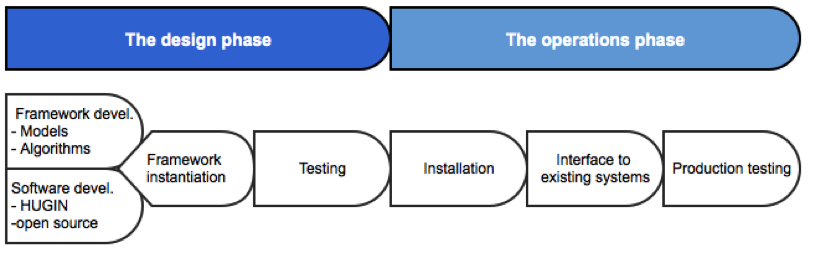
\includegraphics [keepaspectratio,width = 14cm] {REprocess2}
\caption{The table show key steps in the design and operation stages. Notice that each requirement can only be member of one step.} 
\label{REprocess2}
\end{figure}

The design stage contains general functionality requirements for the system, i.e. what the system should do and support.  In figure \ref{REprocess2}, we detail key steps inside this phase. The first step consists of the design of the general framework (models and algorithms) as well as the design and development of the software tools. In a second step, the general framework and software is instantiated for each specific use case. Finally, initial tests of the use case instantiated framework are conducted.  At the design phase, possible design requirements could e.g. address
\begin{itemize}
 \item the scope of the model
 \item the interpretability of the learned models
 \item the extent and type of domain knowledge that can be integrated into the models
 \item documentation
\end{itemize}

The requirements for the operation phase concern the functionality of the deployed system. In figure \ref{REprocess2}, we decompose this phase into three stages: installation, interface to existing systems, and production testing. The requirements for this phase could e.g. address
\begin{itemize}
 \item hardware constraints
 \item interfaces to existing software or data base systems
 \item inference functionality, i.e., what queries the system should be able to answer
\end{itemize}

\subsubsection*{Requirements and work packages allocation}

To make sure that all requirement comply with the document of work that is agreed upon upfront, every requirement is linked with the deliveries that are relevant.  This is clearly a tool to mitigate characteristic one.

\subsubsection*{Requirements prioritization}

In the Amidst RE process, the industrial partners are asked to categorize every requirement as an either must, should or could requirement.  Moreover, they are also asked to give rigorous prioritization of each requirement.  The intention is that the industrial partners are forced to think thoroughly about every requirement and how it relates to solving their problems.  This is a way to mitigate characteristic five.

\subsubsection*{The activities in the AMIDST requirements engineering process}
\label{sec:reprocess}

The activities in the requirement engineering process is carried out in an iterative fashion that is expected to involve a high level of cooperation and interaction between the partners in order to meet all characteristics in subsection \ref{sec:characteristics}. 

In figure \ref{REprocess1}, an illustration of the requirement engineering process for AMIDST is given, which is inspired by \cite{Ebe10}.  In general the process contain five phases, which are discussed below.
\begin{enumerate}
\item Preparation I.  This phase starts at the same time as work package one and ends when the initial template, attachment X1, for the requirement engineering document is finished.  In this template, the requirement engineering process is outlined including definitions of use cases, user groups and how to link requirements with stages in development process.  In order to meet characteristic three, four and five, the use case providers are asked to provide a detailed description of the system context that the AMIDST software is expected to run in, identify user groups, describe use cases and requirements.  In order to meet characteristic four, the requirements are linked with references to stages in the development cycle. 
\item Elicitation. The distribution of the above mentioned template marks the initialization of this phase.  Its aim is to get an initial high-level description of the different use cases and their requirements. This information are specified by the use case providers in collaboration with the academic partners to meet characteristic one, three and four.  Once the use case providers return the present document with the requested information, feedback and informal meetings are expected to clarify and refine the information provided.  At the end of the elicitation phase, the aim is to have a first coherent description of the requirements for each use case provider.
 \item Prioritization. In this phase the use case providers completes an extended version of the document template used in the previous phase. This template is used to link each of the requirements to the relevant work packages and tasks in the AMIDST project to meet characteristic one. Moreover, the template allows the use case providers to provide a more fine grained prioritization of the relevant requirements for the AMIDST framework.  Specifically, the use case providers are asked to rate each requirement in terms of must, should and could and also rate how important the requirement is to them.  
\item Validation. In this phase, the requirements from all use-case providers are collected to get the \emph{big picture}.  This involves a discussion to what extent the requirements can be accommodated. Revisions and negotiations of the detailed requirements are therefore expected.  In this phase, it is important to ensure that characteristic one is met.
 \item Evaluation and Testing. In this phase, the focus is on the elicitation of the evaluation and testing procedures in the AMIDST project. This phase starts with the distribution of a new document template, where the aim is to obtain a high level description of the evaluation and testing methods that is necessary to measure the performance of the AMIDST framework.
\end{enumerate}

\begin{figure}
\centering
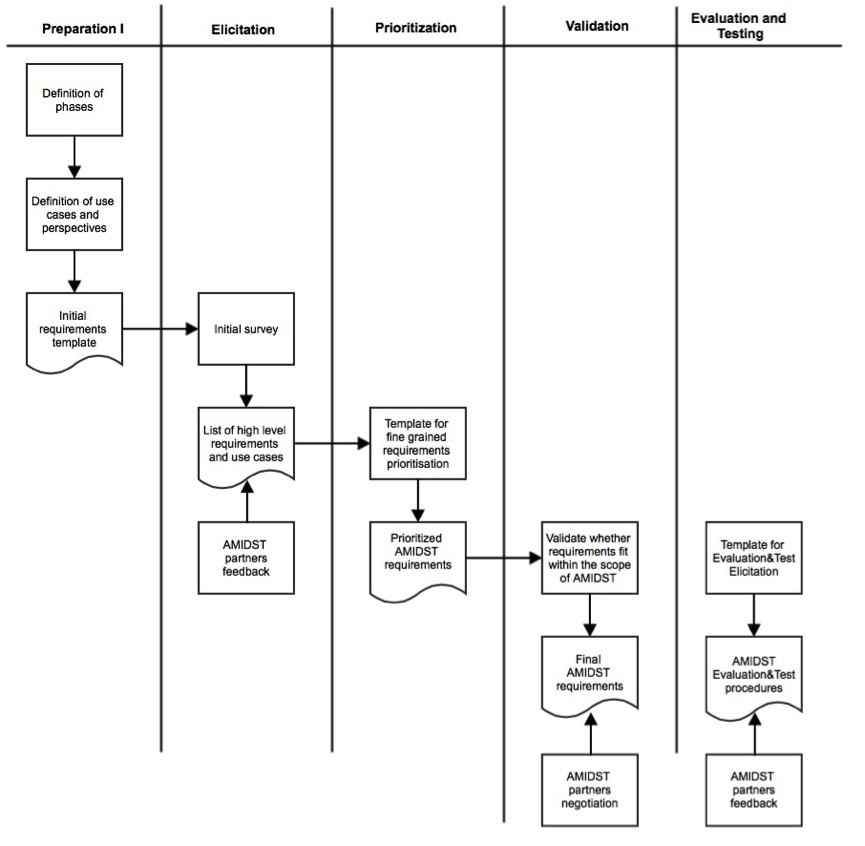
\includegraphics [keepaspectratio,width = 14cm] {REprocess1}
\caption{Description of the five phases in the requirement engineering process in AMIDST.}
\label{REprocess1}
\end{figure}

\section{Realization of the requirements engineering process}
\label{sec:realization}

This part of the report is written in month six when most of the process is conducted.  This section contains a few points on what experiences we have gained in the project so far:

\begin{enumerate}
\item Everyone involved has had a learning experience on many levels.  The industrial partners have learned about probabilistic graphical models, while the academic partners have learned about the industrial domains.  Most participants have increased their knowledge on how to conduct a requirement analysis. 
\item There has only been one meeting where all stakeholders have met, which was the kickoff meeting in Denmark in month three.  Most communication has been done through Skype and email, but also a few face to face meetings have taken place. Most of the communications have been related to clarifications in terms of filling out the template X1.
\item There have been adjustments of the template X1 as the process has proceeded.  Examples of this is adding fields to the requirements so they could be linked to concrete tasks in the AMIDST project or adding columns for rating the importance of a requirement.
\end{enumerate}

\section{Conclusion, observations and reflections}
\label{sec:conclusion}

Based on the lack of agreement in literature and in practice on a unified RE process for small projects, we chose to make our own process.  The approach was to identify the main characteristics in the AMIDST project that is believed to have an impact on the choices for how to conduct the RE process.  The main characteristics are that there is a pre-specified scope in the project, many different stakeholders, the software is supposed to solve very different problems and that the targets are not fully defined.  A use-case driven approach was chosen and we also introduced a document template early in the project to mitigate the above challenges.  The project is not finished yet, so it is difficult to fully evaluate the process today.  However, it is positive that there seem to be a high level of agreement between the partners at this point.

\bibliographystyle{splncs}
\bibliography{re}


\end{document}  